\setchapterimage[6cm]{chapter/human_settlement/human_settlement_main.jpg}
%\setchapterstyle{kao}
\setchapterpreamble[u]{\margintoc}
\chapter[In which settlements of Russia are more scientists born, rural or urban?]{In which settlements of Russia are more scientists born, rural or urban?\protect\footnotemark}
\labch{human_settlement}

\footnotetext{\href{https://commons.wikimedia.org/wiki/File:Detail_of_the_settlement_Vestmannaeyjar-2.jpg}{Human settlement}. 
	Author: \href{https://commons.wikimedia.org/wiki/File:Detail_of_the_settlement_Vestmannaeyjar-2.jpg}{Szilas / 2014 /  Creative Commons Attribution License}.}

The chapter explores the Wikidata object, \wdqName{human settlement}{486972} settlement and its properties. In each of the sections, 
tasks are presented that were solved using SPARQL queries.

A list of settlements was received,
bubble charts were built with the number of population in ``human settlement'' by country.
A chart showing the proportion of the population
living in settlements relative to the entire population of the country.
The chart showed that a high percentage of the population living in localities
falls in agricultural countries, while in more industrialized countries
a smaller proportion of the population lives in human settlement.

To compare rural and urban settlements
built diagrams of the number of scientists, grouped by occupation
and divided by place of birth: rural or urban.

To search for more complete answers to the above tasks
more general classes were found for the object \wdqName{human settlement}{486972}
using the property \wdProperty{31}{instance of}.
The difficulty of the study is due to the lack of a clear typology of human settlements
(for example, from population size) in Russian legislation and in Wikidata.

%
%%%%%%%%%%%%%%%% Exercise 1 %%%%%%%%%%%%%%%%
\marginnote{Calculate how many people per km \textsuperscript{2} live in %~\enwiki{4dNv}{Barabinsk}
and in %~\enwiki{4dNt}{Aleisk}? 
Which of these \emph{human settlements} has the highest population density?
See~\ref{answer: human_settlements_density} on page~\pageref{answer: human_settlements_density}.}

%%%%%%%
\section{List of ``human settlement''}

Let's build a list of all human settlements using the query~\ref{lst:human-settlement1}.

\begin{lstlisting}[ language=SPARQL, 
                    caption={List of all human settlements. \num{411393} items received in 2017. SPARQL query:\href{https://w.wiki/4d7x}{https://w.wiki/4d7x}},
                    label=lst:human-settlement1,
                    texcl 
                    ]
# List of all human settlements
SELECT ?hum ?humLabel WHERE{
  ?hum wdt:P31 wd:Q486972. # instance of human settlement
  SERVICE wikibase:label{bd:serviceParam wikibase:language "ru,en"}
}
\end{lstlisting}%

In 2021, it turned out to be impossible to get a list of human settlements
due to the large number of objects and, therefore, the query takes too long~\ref{lst:human-settlement1}.
To calculate the number of all human settlements, refer to the \lstinline|COUNT()|
in the request~\ref{lst:human-settlement2}.

\index{SPARQL!COUNT!Number of human settlements}
\begin{lstlisting}[ language=SPARQL, 
                    caption={Number of human settlements. \num{411393} items received in 2021. SPARQL query:\href{https://w.wiki/4d7s}{https://w.wiki/4d7s}},
                    label=lst:human-settlement2,
                    texcl 
                    ]
# Number of human settlements
SELECT (COUNT(?hum) AS ?count) WHERE {
  ?hum wdt:P31 wd:Q486972. # instance of human settlement  
}
\end{lstlisting}%

Among domestic settlements on Wikidata,
which correspond to the articles of the Russian Wikipedia,
almost empty are, for example,
former village \wdqName{Borisovo}{4093951} (3 properties)
and \wdqName{Brigadier forestry}{21668554} (4 properties).

According to the ProWD service
among domestic settlements
\wdqName{Yalta}{128499} has the most properties (36).
The world leader is \wdqName{Tokyo}{1490} (73 properties)\sidecite{humansettlements_ProWD}.

%%%%%%%
\section{List of countries by total population}

Using the query~\ref{lst:human-settlement3}
Let's build an ordered list of countries according to the total number of people living in ``human settlement''.

\index{SPARQL!SUM!List of countries by population in ``human settlement''}
\index{SPARQL!GROUP BY!List of countries by population in ``human settlement''}
\lstset{numbers=left, firstnumber=1, frame=single}
\begin{lstlisting}[ language=SPARQL, 
    caption={List of countries by population in settlements. The result contained \num{161} countries in 2017 and \num{213} countries in 2021. SPARQL query:\href{https://w.wiki/4d9M}{https://w.wiki/4d9M}},
    label=lst:human-settlement3,
    texcl 
                  ]
# List of countries by population in settlements
SELECT ?country ?countryLabel (SUM(?population) as ?sumPopulation)
WHERE {
  ?hum wdt:P31 wd:Q486972;  	# instance of human settlement
       wdt:P17 ?country;    	# in the ?country
       wdt:P1082 ?population. # has ?population
  SERVICE wikibase:label{bd:serviceParam wikibase:language "ru,en"}
}
GROUP BY ?country ?countryLabel 
ORDER BY DESC (?sumPopulation)
\end{lstlisting}%

To calculate the number of population by country
use the command \lstinline|SUM()| in the second line of the query~\ref{lst:human-settlement3}.
To group settlements by country
use the command \lstinline|GROUP BY| on the ninth line of the same query.

Bubble chart in Figure~\ref{fig:human-settlement-1}
shows the ratio of countries by population in ``human settlement'' in 2017.

\begin{figure}
\centering
	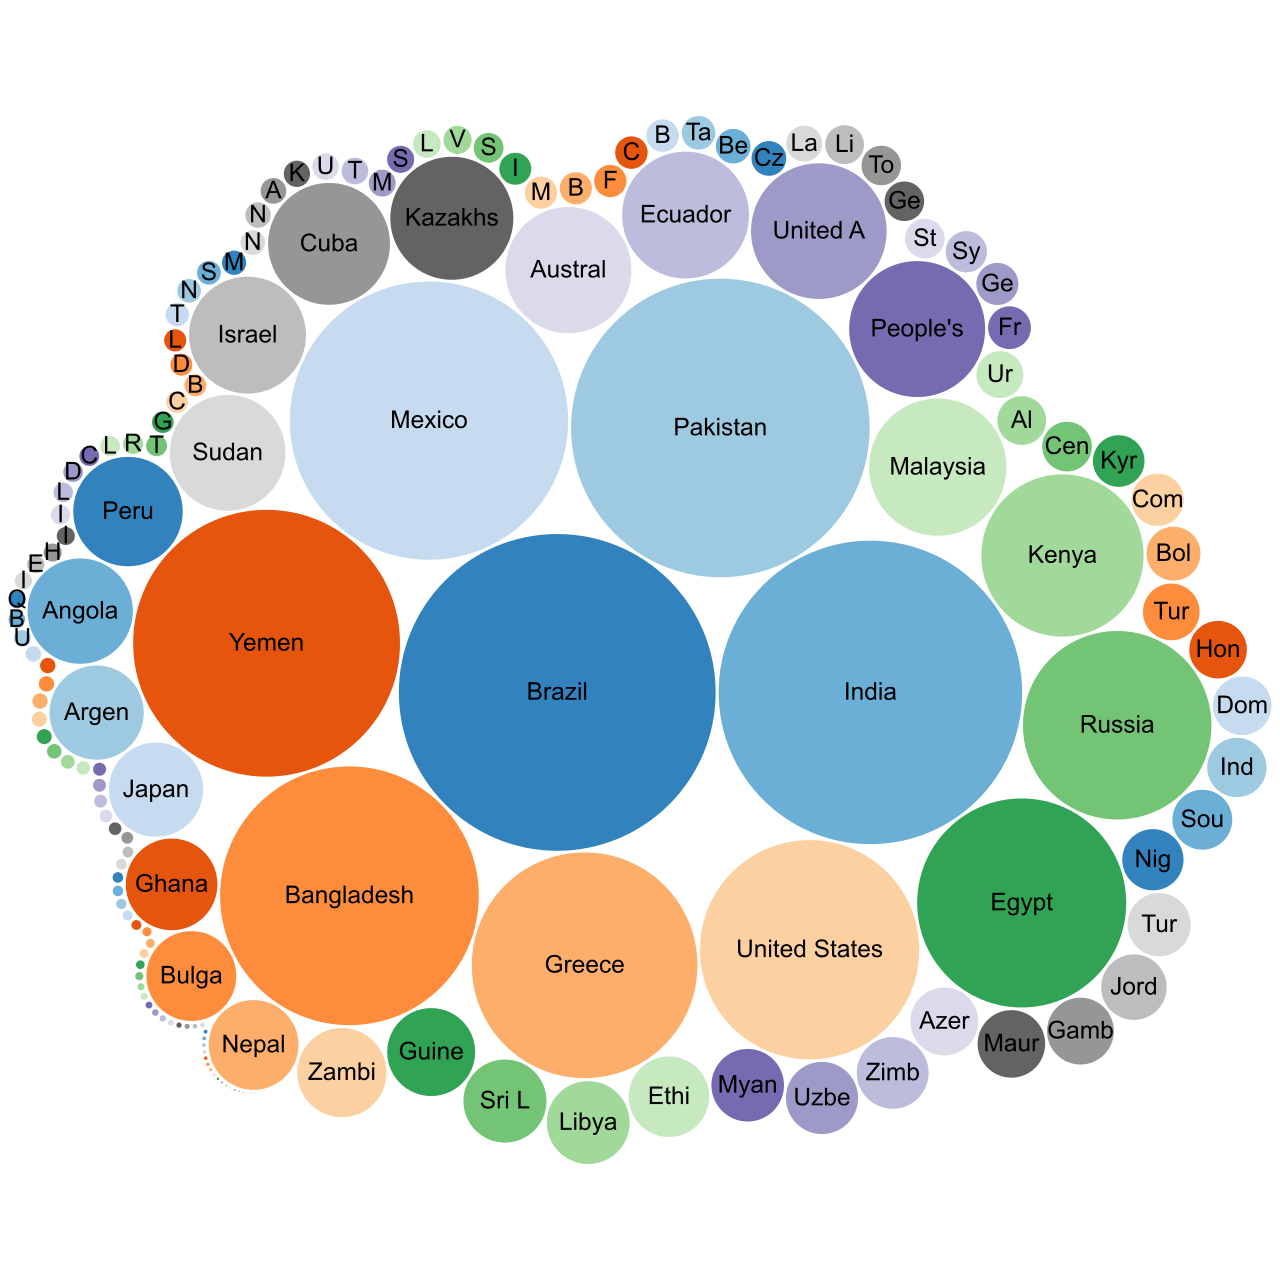
\includegraphics[width=0.9\linewidth]{./chapter/human_settlement/AnnaBubbleHumanSettlement.jpg}
	\label{fig:human-settlement-1}
    \caption[Bubble chart for the total population in ``human settlement'', 2017.] {Bubble chart for the total population living in ``human settlement'' for 2017. The size of the bubble corresponds to the number of people living in ``human settlement'' of one country. SPARQL query: \href{https://w.wiki/4dAv}{https://w.wiki/4dAv}}
\end{figure}

\begin{figure}
\centering
	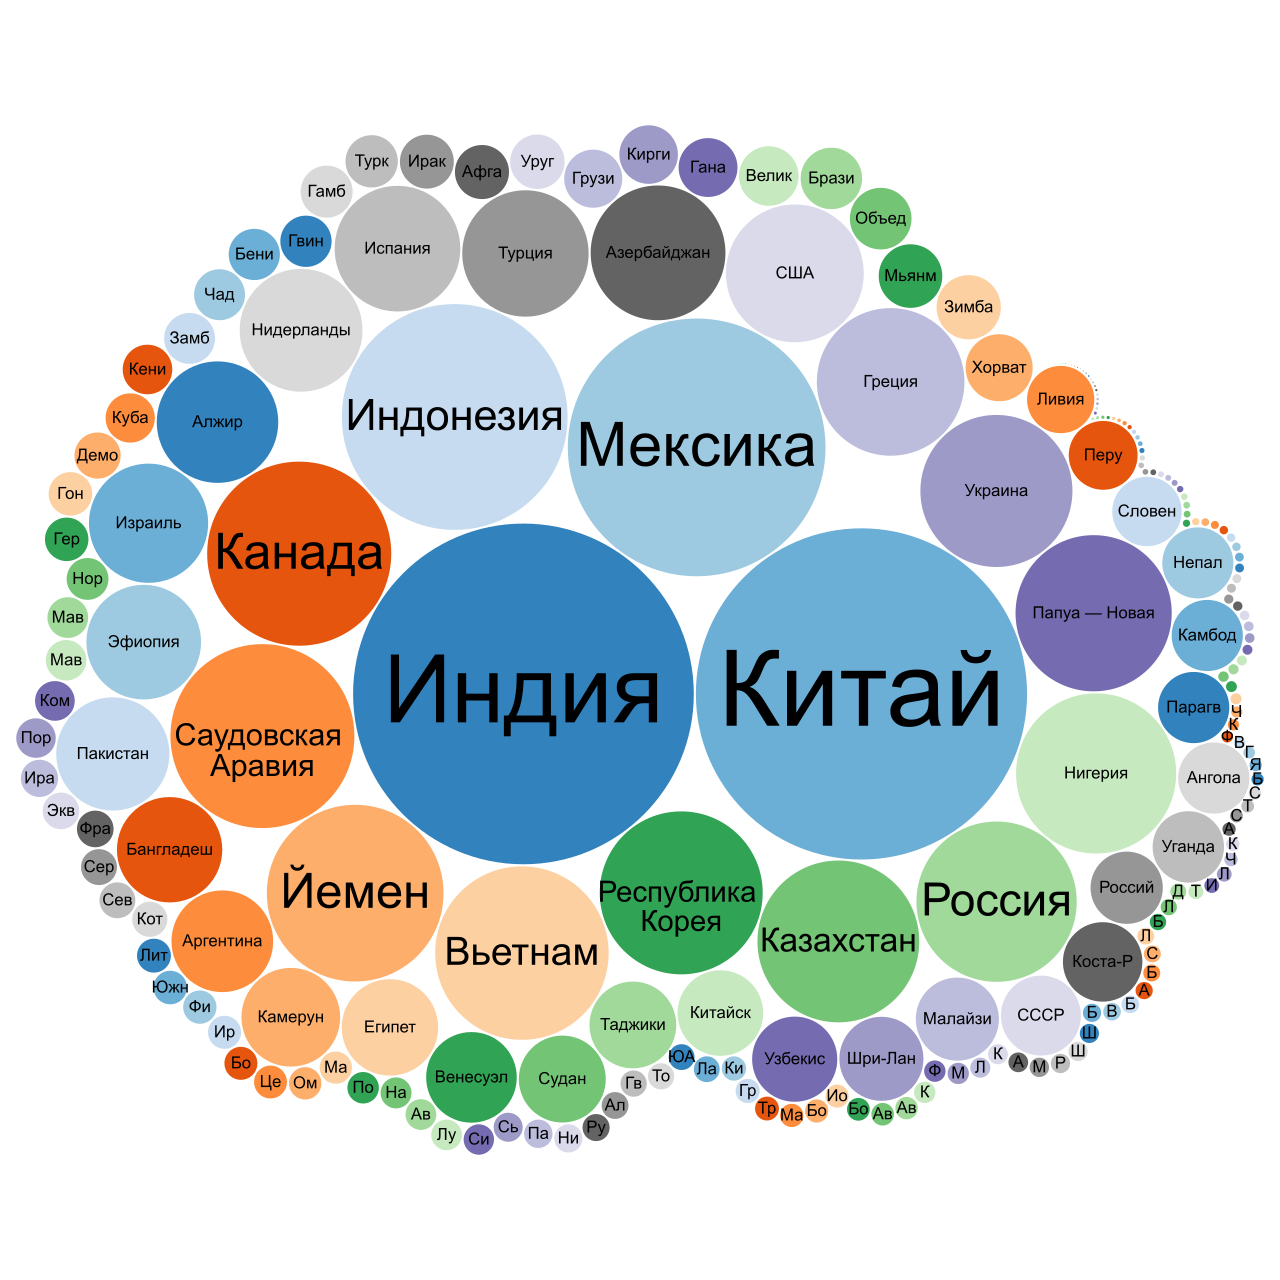
\includegraphics[width=0.9\linewidth]{./chapter/human_settlement/LeonidBubbleHumanSettlement.jpg}
	\label{fig:human-settlement-2}
	\caption[Bubble chart for the total population in ``human settlement'', 2021.] {Bubble chart for the total population living in ``human settlement'' for 2021. The size of the bubble corresponds to the number of people living in ``human settlement'' of one country. SPARQL query: \href{https://w.wiki/4dAv}{https://w.wiki/4dAv}}
\end{figure}

%%%%%%%%%%%%%%%% Exercise 2 %%%%%%%%%%%%%%%%
\begin{marginfigure} [0.0cm] {%

\includegraphics [width = 0.9\linewidth] {./chapter/human_settlement/Aznakeevskii_rayon_gerb.png}}
   \caption {Is the coat of arms of a domestic or foreign human settlement shown in the picture?}%
   \label {fig:flag_question_human_settlements1}%
\end{marginfigure}
\marginnote {
See~\ref{answer:flag_human_settlements} on page~\pageref{answer:flag_human_settlements}.
}

In 2017, most of the population lived in ``human settlement'':
\wdqName {Brazil} {155} (\num {12} millions),
\wdqName {Pakistan} {843} (\num {10} millions),
\wdqName {Mexico} {96} (\num {8} millions),
\wdqName {Yemen} {805} (\num {8} millions),
\wdqName {India} {668} (\num {7} millions) and
\wdqName {Bangladesh} {902} (\ num{7} millions).

In Figure~\ref{fig:human-settlement-2}, you can see the list of countries for 2021:
\wdqName {India} {668} (\num {30} millions),
\wdqName {China} {148} (\num {28} millions),
\wdqName {Mexico} {96} (\num {17} millions),
\wdqName {Indonesia} {252} (\num {13} millions),
\wdqName {Canada} {16} (\num {9} millions) and
\wdqName {Saudi Arabia} {851} (\num {9} millions).

So, the results of the query~\ref{lst:human-settlement3} in 2017 and 2021 differ significantly.
Based on these results, it turns out that in four years
in the settlements of India has increased by 23 million people.

%%%%%
\subsection{Completeness of Wikidata}

Human settlement~--- is the common name for places with permanent residents\sidecite{Humansettlements_Dictionary}.
According to the editors of Wikidata, the concept of a locality includes cities, villages, hamlets
and others \marginnote [12pt] {The complete list can be seen in the section ``List of classes accompanying ``human settlement'' in the property ``instance of'''' on page~\pageref {human-settlement:tag1}.}.
Accurate information on the number of human settlements in the world was not found.
Therefore, we will check the completeness of the human settlements that are in Wikidata.
and which were used to solve the problem.
In the tasks above, we used the \wdProperty{1082}{population size} property and
\wdProperty{17}{state} (binding to the country).
Based on this, we divide the completeness check into subtasks:
\begin {enumerate}
  \item Check if the property ``population size'' is full.
  \item Check of attachment to the state.
\end {enumerate}

%%%%%
\subsection{Checking the occupancy of the property ``population''}

For such a check, write \href{https://w.wiki/4FUz}{SPARQL query}\sidenote {
%
In 2017, the request returned \num{372997} settlements
with the property ``population size'' empty.
The same request in 2021 yielded \num{507078} such settlements.
SPARQL query link: \href{https://w.wiki/4FUz}{https://w.wiki/4FUz}%
},
which will display settlements
with an empty property \href{http://www.wikidata.org/entity/P1082}{population size}.
Making calculations, we find that only 9.3\% of the world's settlements
the property ``population size'' for 2017 is indicated.
In 2021, we get 11.2\% of the world's settlements with a filled property ``population size''.
So, simultaneously with the increase in the number of settlements in Wikidata
he share of points with the filled property ``population size'' is growing.

%%%%%
\subsection{Verification of state supplies}

%%%%%%%%%%%%%%%%% Exercise 2 %%%%%%%%%%%%%%%%%%
\begin{marginfigure} [0.0 cm]
{
\includegraphics [width = 0.8\linewidth] {./chapter/human_settlement/Coat_of_Arms_of_Asbest_(Sverdlovsk_oblast).png}}
    \caption {Is this the emblem of a settlement in Russia or other countries? \newline%
See~\protect\ref{answer:flag_human_settlements} on page~\protect\pageref{answer:flag_human_settlements}.}
    \label {fig:flag_question_human_settlements2}%
\end{marginfigure}

Now let's see the settlements,
in any country
using \href{https://w.wiki/4FV8}{SPARQL query} \footnote {%
%
In 2017, there were \num{8427} objects that did not include a record in any country.
In 2021, there are already more such objects~--- \num{27824}.

SPARQL query: \href{https://w.wiki/4FV8}{https://w.wiki/4FV8}%
}.

The query results show that the numeric value is not tied to a country that has been growing over the years.
Therefore, associated with settlements and countries,
not completely in terms of coverage, even relative to those already in Wikidata.

%%%%%
\section {Percentage of the country's population living in ``human settlement''}

Let's build an ordered list of countries in terms of the proportion of the population (in percent) living in \href{http://www.wikidata.org/entity/Q486972} {human settlements}, relative to the number of all inhabitants of the country (listing ~\ref{lst:human-settlement6}).

%%%%%%%%%%%%%%%%% Exercise 2 %%%%%%%%%%%%%%%%%%
\begin{marginfigure} [0.0 cm]
{
\includegraphics [width = 0.8\linewidth] {./chapter/human_settlement/Loučovice_CoA.jpg}}
    \caption {The coat of arms of the locality of which country is depicted? \newline%
See~\protect\ref{answer:flag_human_settlements} on page~\protect\pageref{answer:flag_human_settlements}.}
    \label {fig:flag_question_human_settlements3}%
\end{marginfigure}

\index{SPARQL!SUM!The ratio of the number of people living in settlements to the number of all people in the country}
\begin{lstlisting}[ language=SPARQL, 
                    caption={The ratio of the number of people living in settlements to the number of all people in the country. The result contained \num{158} countries in 2017 and \num{206} countries in 2021. SPARQL query:\href{https://w.wiki/4dE3}{https://w.wiki/4dE3}},
                    label=lst:human-settlement6,
                    texcl 
                    ]
# An ordered list of the ratio of the number of people living in 
# "human\_settlement" to the number of inhabitants in the country.
SELECT ?country ?countryLabel ?proportionPopulation WHERE {
 SELECT ?country ?countryLabel (SUM(?population / ?pop) 
        as ?proportionPopulation) WHERE {
  ?hum wdt:P31 wd:Q486972;    # instances of human settlement  
       wdt:P17 ?country;         # has ?country 
       wdt:P1082 ?population.    # has ?population
  ?country wdt:P1082 ?pop.    # population in the country
  SERVICE wikibase:label{bd:serviceParam wikibase:language "ru,en"}
 }
 GROUP BY ?country ?countryLabel
}
ORDER BY ?proportionPopulation
\end{lstlisting}%
